\chapter{Machine Learning Approaches}

The QG-Net model is not a complete end to end question generation model. One of
the preprocessing steps as required by the model, of tagging possible answer
words in a given test sentence is not performed by the model. To perform this
preprocessing task, various machine learning models were tried. Some of the
approaches giving relatively the best results have been discussed below:

\section{Dataset generation:}

For the training, validation and testing the machine learning models SQUAD
dataset was used. Dataset contains files which have context paragraphs,
questions, the location of starting and ending characters which form the answer
and few more fields in json format. The dataset was parsed into csv files for
model development and data analysis purposes. 

\section{Models:}

\subsection{Model using LSTM}
For generating questions, a model is required which can tag possible answer
words in a sentence. To accomplish this task, the understanding the context is
necessary and hence a RNN based approach was finalised. To overcome the common
problem of vanishing gradient, a LSTM neural network was also applied. LSTM
traverses the sentence word by word and can understands the complete context of
the sentence - a fundamental requirement of the task. 2 dense layers using ReLU
and Softmax activations, respectively, are used.
The last dense layer has 2 nodes as the output of this model. The two numbers
for each word represent the probability of that word being the answer. Sum of
these probabilities is 1 so categorical cross entropy loss function is used in
this case.

\subsubsection{Softmax activation function}
The softmax function is a function that takes as input a vector of K real
numbers, and normalizes it into a probability distribution consisting of K
probabilities. That is, prior to applying softmax, some vector components could
be negative, or greater than one; and might not sum to 1; but after applying
softmax, each component will be in the interval ( 0 , 1 ), and the components
shall add up to 1, so that they can be interpreted as probabilities.
Categorical Cross Entropy:

\begin{figure}
	\caption{Softmax Activation Formula}
	\centering
\includegraphics[width=10cm]{6.png}
\end{figure}

The results of this model were not encouraging as the probability that a word is
an answer word was far too less as compared to probability that it is not. So no
word of the test sentence was tagged as an answer word. On analysis it was found
that this model  was extremely heavy for a simple task of tagging answer words.
Another reason as identified was that training a LSTM requires very large
dataset. Hence, it was decided to try with a simple linear layer model.

\subsection{Model simple Dense Layer}
A simple model containing Dense layers and Sigmoid activation function is built.
The output of the model is a binary string which contains 0s and 1s where 1
indicates that the word is a possible answer word and 0 being not an answer
word.

This is a multiclass multilabel task which means more than one output classes
(multi-word output) are present and more than one word can be tagged as answer
i.e. sum probabilities of words being tagged as answer should not be 1. To
achieve this sigmoid activation function with binary cross entropy loss are
used.

\begin{figure}
	\caption{Sigmoid Function}
	\centering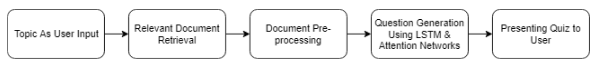
\includegraphics[width=10cm]{7.png}
\end{figure}

\begin{figure}
	\caption{Binary Cross-Entropy Formula}
	\centering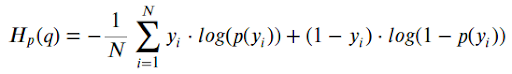
\includegraphics[width=10cm]{8.png}
\end{figure}

\subsubsection{Adam optimizer}
Adam is an optimization algorithm that is used instead of the classical
stochastic gradient descent procedure to update network weights iterative based
in training data. In classical stochastic gradient, a single learning rate for
all weight updates are maintained and the rate does not change during training.
But in adam optimizer, the learning rate is maintained for each network weight
and separately adapted as learning unfolds.

On testing the model on various inputs, it was found out that some words of the
sentences were tagged as answer words and this was given as input to the QG-Net
algorithm. On analysis of the generated questions, it was found that some of the
questions had scope of improvement in terms of getting a natural feel to the
question or in tagging the probable answer words correctly.

